\documentclass{article}
\usepackage[numbers,sort&compress]{natbib}
\usepackage{graphicx}
\usepackage{amsmath}
\usepackage{amssymb}
\usepackage{bm}
\usepackage{color}
\begin{document}
\begin{abstract}
Recently we investigated the applicability and parameters choice for the two-dimensional case
Bretherton problem using the lattice Boltzmann method (LBM) {\color{red} Give citation here}. This
paper is the continuation of the previous work and is focused on the three-dimensional case to
validate the LBM for simulation of phenomena for rectangular and square capillaries in the
moderate range of Capillary number parameters. 
\end{abstract}
\section{What to examine}
I suggest to examine first of all the application of the LBM for really small capillary number,
where it's not possible to resolve the interface. In this case one should find the asymmetric
radiuses for the droplet, the difference should be around $10$ percent. While applying the forcing
it should come to the spheric shape. As well we need to examine the capillary number dependancy on
the length and suggest to examine some axicentric factors for rectangular channels.

\section{Introduction}
While for two-dimensional Bretherton flow the results are usually limited to the circular shape and
only some of them are for the plane-symmetric case \cite{giavedoni-numerical,heil-bretherton},
vast number of experimental results and simulations are available for the three-dimensional case.
It was found that the for rectangular and/or square shaped capillaries there is a transition for
certain capillary number, where the flow changes from the non axisymmetric to axis symmetric case.
The number is indicated in a number of works of as $\hat{Ca}=0.04$ \cite{cerro-bubble-train},
$\hat{Ca}=0.1$
\cite{cerro-space}, $\hat{Ca}=0.033$ \cite{heil-threedim}. If the capillary number is larger than
the critical capillary number, i.e. $Ca>\hat{Ca}$, then the flow becomes axisimmetric with the
radius of the droplet dependant on the capillary number.

The following pictures summarize the radius of deposited liquid on the capillary length.
\citet{heil-threedim} performed three-dimensional simulations for circular shaped and for the
square shaped capillaries and gravitational effects for circular shaped capillaries. The results for
square capillaries are shown in Fig.\ref{fig:heil:three:dim}. On another hand authors performed
numerical simulations for rectangular shaped capillaries. It was found that aspect ratio $\alpha$
allows to put all the different curves on one purely empirical curve through the following parameter
$s_{\infty}=r_{\infty} \alpha^{-1/2}$, where $r_{\infty}$ is the aximsymmetric bubble radius
infinitely far behind the bubble tip and can be calculated from the flow rate in the computational
domain:
\begin{equation}
r_{\infty}=2\sqrt{(a-Q)/\pi}.
\end{equation}
It is also indicated that for $\alpha\geq\hat{\alpha}=2.04$ the interface can not make up the
axisymmetric case. The $s_{\infty}$ dependency on $\alpha$ is shown in Fig.
\ref{fig:heil:three:dim}.
\begin{figure}
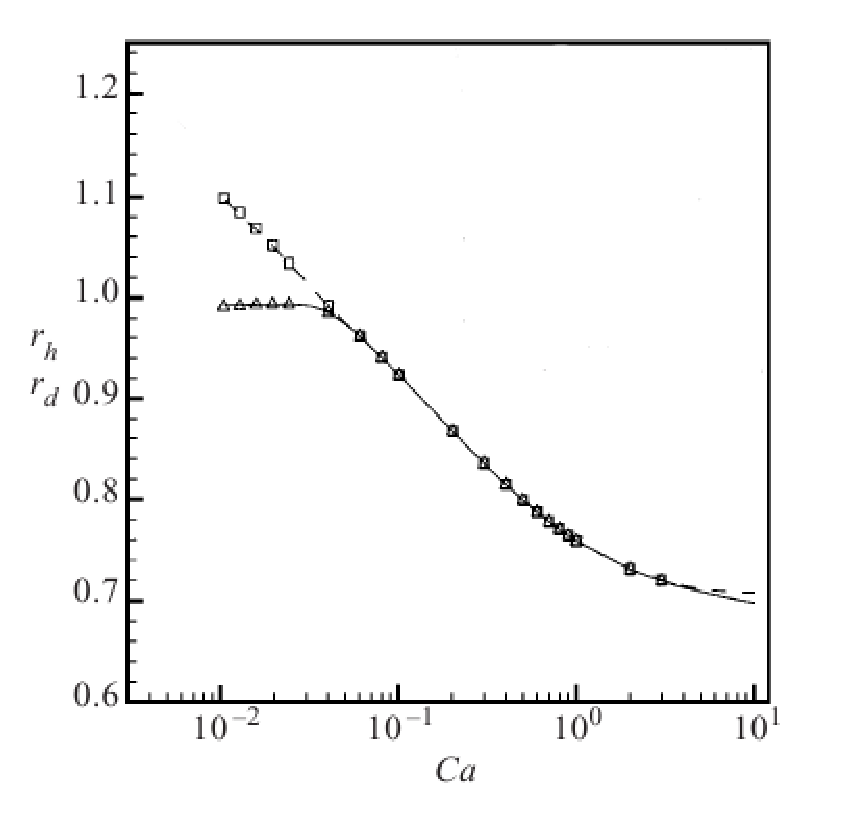
\includegraphics[width=0.47\textwidth]{Figures/capillary_width_heil.eps}\hfill
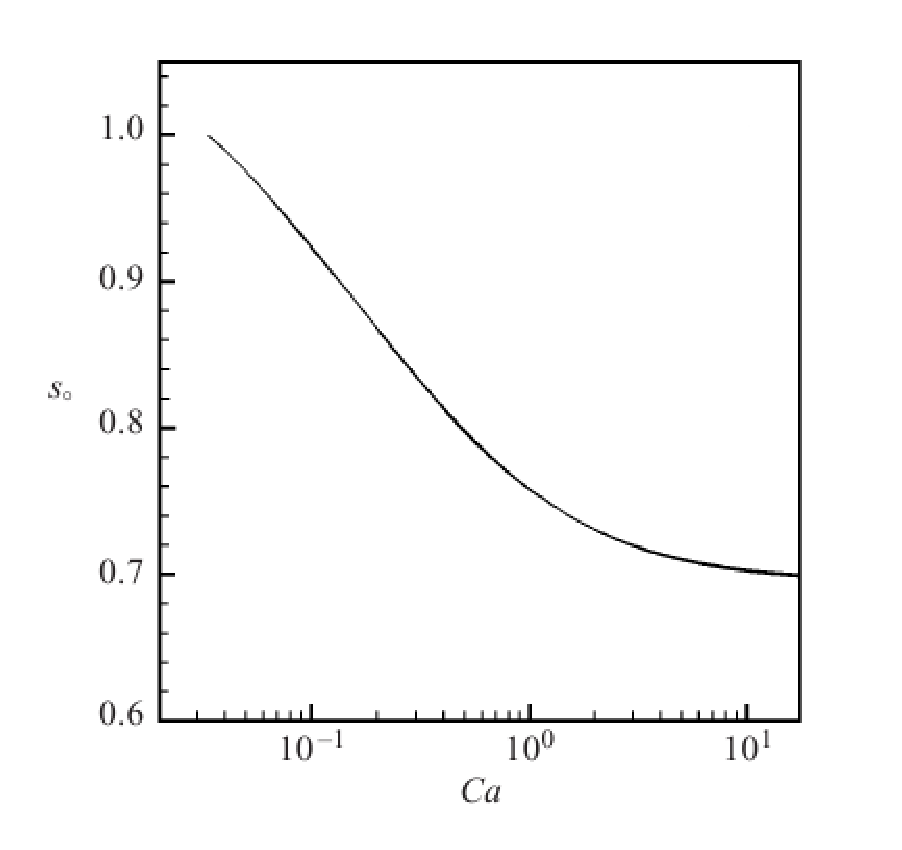
\includegraphics[width=0.47\textwidth]{Figures/capillary_rectangular_width_heil.eps}\\
\caption{\citet{heil-threedim} results for the variation of the deposited liquid for the range of
capillary number. One can see the asymmetry between diagonal and axis diameter for the capillary
number $Ca\leq\hat{Ca}=0.04$.\label{fig:heil:three:dim}}
\end{figure}
There is also interesting thing to track down is the recirculating regime for flow fields. It is
known that for certain capillary number the streamlines either go around the bubble or create the
circulating regime in front of the bubble. The calculation ({\color{red} or analytical data? Look
at White 1991, pp. 119-120. As well put figures if there is a space from Heil et al.}) are presented
in Table \ref{table:recirculation:data}.
\begin{table}
\begin{tabular}{c|c}
$\alpha$& $Ca_{T}$\\
\hline
1& 0.691\\
1.1 & 0.688\\
1.3 & 0.666\\
1.5 & 0.631\\
\end{tabular}
\caption{The results for the recirculation region.\label{table:recirculation:data}}
\end{table}

\citet{shikazono-square} obtained a lot of different results for the deposition length versus the
capillary number variation for FC-40/air, ethanol/air and water/air experiments. All of them are
presented in Fig. \ref{fig:deposition:han}.
\begin{figure}
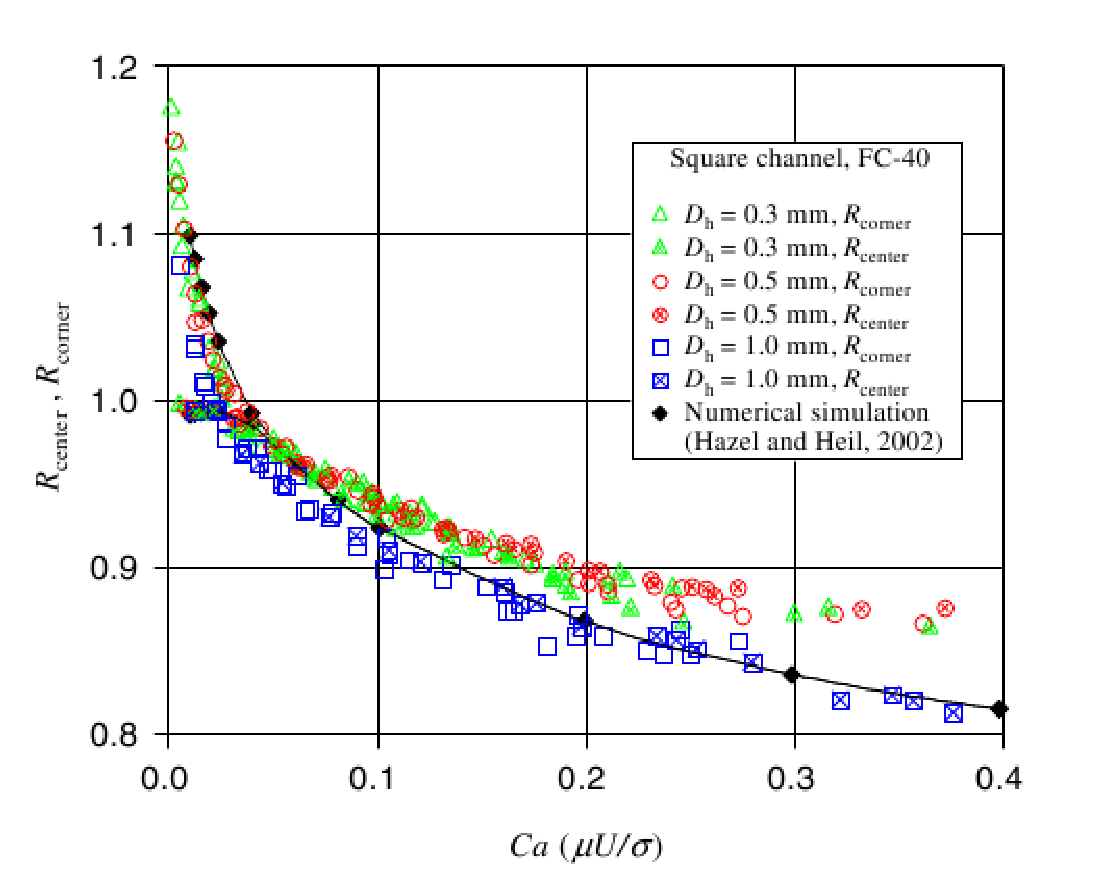
\includegraphics[width=0.33\textwidth]{Figures/han_capillary_fc40_air.eps}\hfill
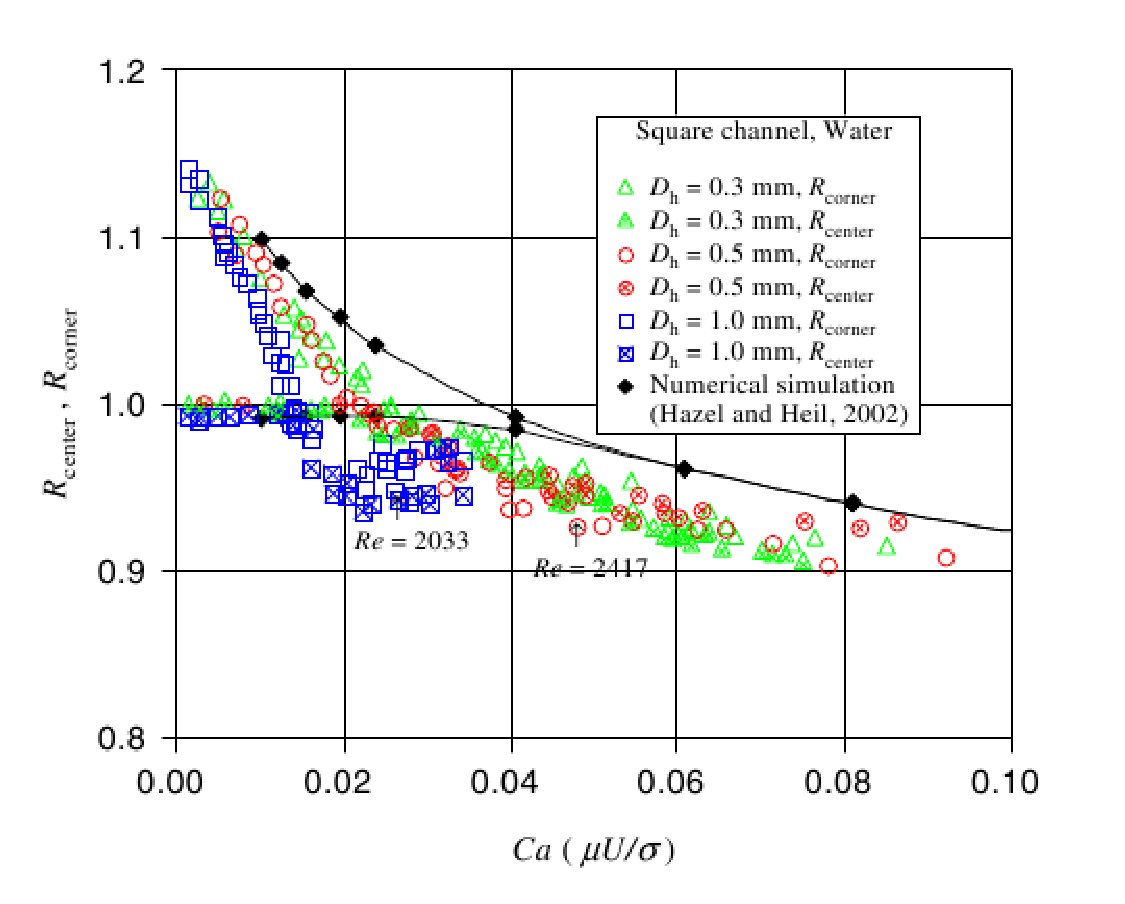
\includegraphics[width=0.33\textwidth]{Figures/han_capillary_water_air.eps}\hfill
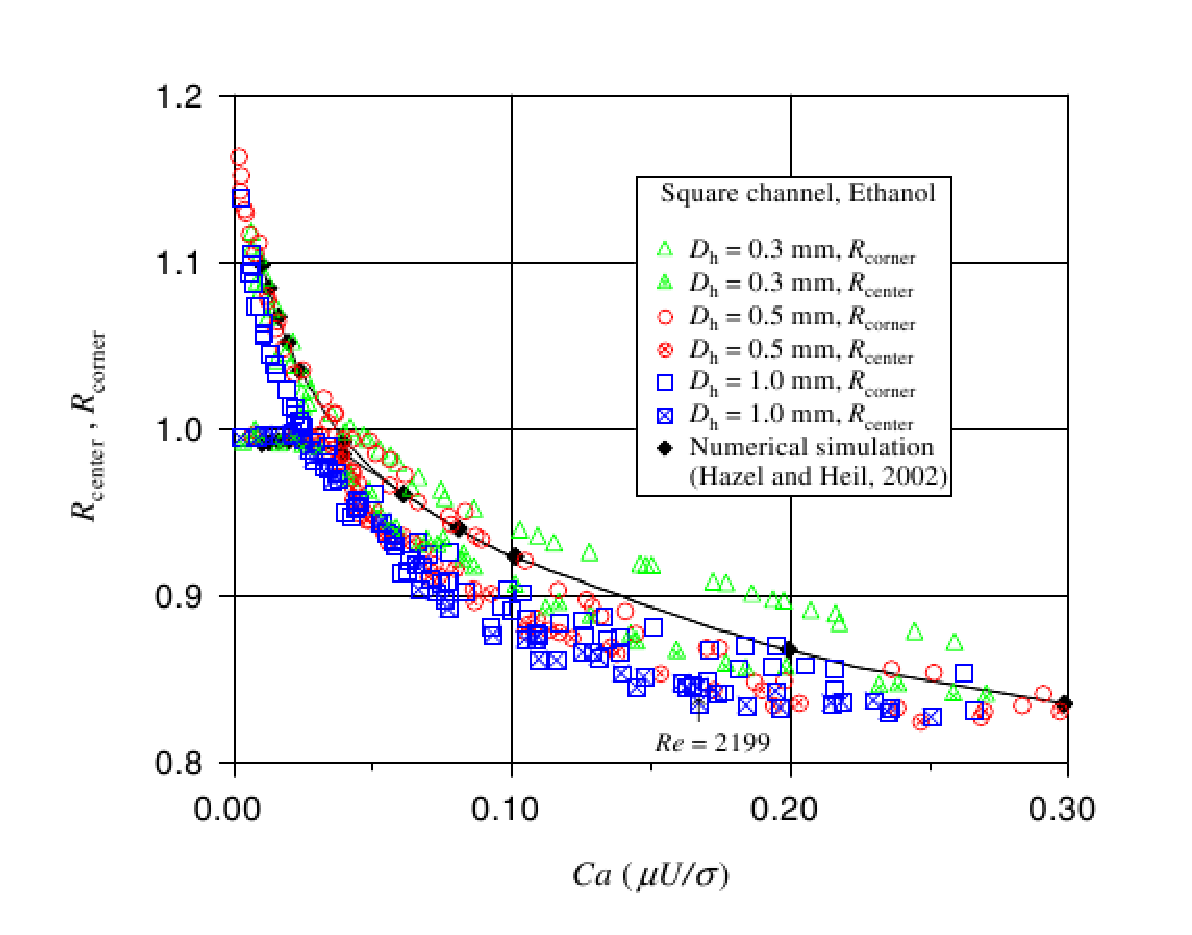
\includegraphics[width=0.33\textwidth]{Figures/han_capillary_ethanol_air.eps}\\
\caption{Han results. \label{fig:deposition:han}}
\end{figure}

\section{Variation bubble length}
The work of \cite{heil-threedim} shows the variation of the bubble thickness through the length of
bubble. The length variation is presented in Fig. \ref{fig:thickness:variation:ca:ten}
\begin{figure}
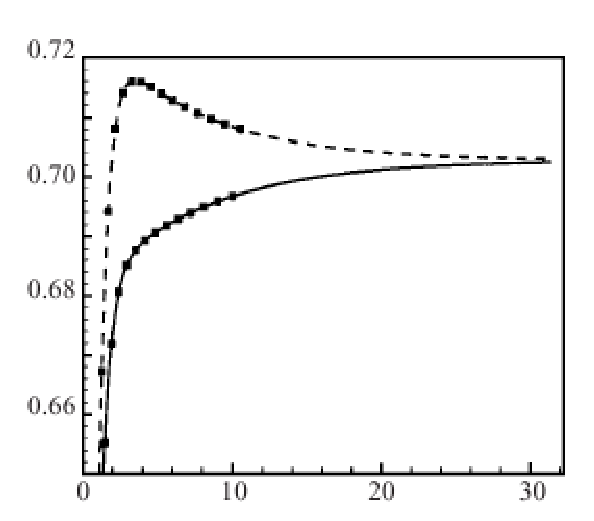
\includegraphics[width=0.97\textwidth]{Figures/variationoverlength.eps}
\caption{The variation of the bubble length for capillary number $Ca=10$. The x-axis scaled to
half-width of the microchannel height.  \label{fig:thickness:variation:ca:ten}}
\end{figure}
We want to obtain the same characteristics as indicated in Fig.
\ref{fig:thickness:variation:ca:ten}. One can see that the difference between diagonal radius and
usual radius is of order of $4\%$. That means it's 2 percent of the channel height. If the
simulation is conducted by the grid $50\mathrm{x}50$ in the cross section that means that we will
see the difference in one grid node. Therefore the grid is $52\mathrm{x}52\mathrm{750}$. Here we
conduct a scaling:
\begin{equation}
Ca=\frac{\mu_{liq} U_{bubble}}{\gamma}
\end{equation}
The parameters for the binary liquid problem are chosen as $A=0.04$ and $k=0.01$. Therefore the
surface tension is:
\begin{equation}
\sigma = \sqrt{\frac{8 k A}{9}}=0.0596
\end{equation}
The relaxation times for liquid and gas are taken as, $\tau_{gas}=0.7$ and $\tau_{liq}=2.5$,
therefore the viscosities ratio is $10$.
\begin{equation}
\begin{aligned}
&10=\frac{\frac{2}{3} U_{bubble}}{0.0596},
&U_{bubble}=0.894
\end{aligned}
\end{equation}
which is quite high for the lattice Boltzmann method. We can decrease the ratio by scaling
parameters $k$ and $A$ while keeping the interface thickness. Let us choose parameters as $k=0.001$
and $A=0.004$, therefore the mobility should be adjusted to address the issue with small parameters
and small surface tension in this case. It parameters are chosen as $A=0.004$ and $k=0.001$ then
the velocity of the bubble is  $0.0894$. Therefore we can adjust the pressure gradient to plug it
into the bubble initialization:
\begin{equation}
\frac{\mathrm{d}P}{\mathrm{d}x}=\frac{8}{N_y^2} \gamma Ca=0.0001907,
\end{equation}
which is quite high for lattice Boltzmann simulations. Therefore probably one more time the surface
tension needs to be reduced. {\color{red} Many authors state that increasing mobility kills the
proper results of simulations}. 
The film thickness as it is seen from the picture is taken as $70$ percent of the half channel.
Therefore the initalization width is $0.15*50=7.5$. 

\section{Non-axisymmetric case}
That could be fucking difficult. For example according to \cite{heil-threedim} for the capillary
number $Ca=0.01$, the radiuses converge as $r_h=0.99$ and $r_d=1.1$. Therefore one needs to resolve
as the $0.5\%$ of whole channel width to see the difference. That certainly implies so large grid
that can kill the simulation at least $200x200x3000$. However, we can refer to artificially made
interface as $1-2$ lattice Boltzmann units but keeping the capillary number as it is required. In
this case we can refer like we can't resolve the interface but we can certainly to attribute it to
the wall gradient as extreme case. The dimnesionalization case is therefore as follows:
\begin{equation}
Ca=\frac{\mu_{liq} U_{bubble}}{\gamma},
\end{equation}
therefore let us pick up the same parameters as for the previous case and just change use the
pressure gradient reduced by $1000$ as $Ca=10$ and $Ca=0.01$ are different. 
Let us wait for simulation.

\section{Capillary number region}



\section{Simulation setup}


\bibliographystyle{unsrtnat}
\bibliography{paper}
\end{document}


